\documentclass[11pt]{article}

\title{Relazione 4: Soluzione numerica Problemi di Cauchy}
\author{Antonio Michele Miti}

\usepackage{amsmath}
\usepackage{amsfonts}
\usepackage[utf8]{inputenc}
\usepackage[italian]{babel}
\usepackage{listings}
\usepackage{textcomp}
\usepackage{graphicx}
\usepackage{subfigure}
\usepackage{caption}
\usepackage{latexsym}
\usepackage{epstopdf}
\usepackage{eepic,epic,eepicemu}
\usepackage{color}
\pagestyle{headings}
\definecolor{listinggray}{gray}{0.9}
\definecolor{lbcolor}{rgb}{0.95,0.95,0.95}
\lstset{
	backgroundcolor=\color{lbcolor},
	rulecolor=,
	language=C++,
        basicstyle=\scriptsize,
        upquote=true,
        aboveskip={1.5\baselineskip},
        columns=fixed,
        showstringspaces=false,
        extendedchars=true,
        breaklines=true,
        prebreak = \raisebox{0ex}[0ex][0ex]{\ensuremath{\hookleftarrow}},
        frame=single,
        showtabs=false,
        showspaces=false,
        showstringspaces=false,
        identifierstyle=\ttfamily,
        keywordstyle=\color[rgb]{0,0,1},
        commentstyle=\color[rgb]{0.133,0.545,0.133},
        stringstyle=\color[rgb]{0.627,0.126,0.941},
}
\addtolength{\hoffset}{-1.25cm}
\addtolength{\voffset}{-1.80cm}
\addtolength{\textwidth}{1cm}
\addtolength{\textheight}{3.80cm}




\begin{document}
\maketitle
\begin{abstract}
In questo articolo si intende mostrare come implementare alcuni algoritmi numerici per il calcolo della soluzione dei problemi di Cauchy di primo ordine stimandone graficamente l'ordine di approssimazione.

Inoltre viene descritta la possibile estensione di tali metodi ad equazioni differenziali ordinarie ad ordini superiori al primo al fine di applicarlo allo studio della dinamica del "Pendolo Caotico".

L'interesse di questo sistema fisico sta nella sua forte dipendenza dai parametri inziali, tale da mostrare un comportamento pseudo-caotico attorno a particolari valori critici.
\end{abstract}

%\tableofcontents


\section{Introduzione}

Dato il problema di Cauchy
	\begin{equation}
	\left\{ 
			\begin{array}{rcl}
 			\dot{y(t)} &=& f(t,y(t))\\
 			y(t_{0}) &=& y_{0} \\
  			\end{array} \right.
	\end{equation}

di soluzione
	\begin{equation}
	y(t)=y_{0}+\int_{t_{0}}^{t}f(x,y(x)) \, \textrm{d} x
	\end{equation}
si è interessati a trovare una soluzione numerica del problema.

In altre parole si cerca di ottenere con una certa approssimazione un samplaggio, valutazione della funzione in un numero discreto $\{ t_{i}\} _{i\in \textrm{N}}$ di punti del dominio, della funzione soluzione.

Analiticamente vale che
	\begin{equation}
		y(t_{i+1})=y_{0}+\int_{t_{i}}^{t_{i+1}}f(x,y(x)) \, \textrm{d} x 
		=y_{0} + h_{i}\int_{0}^{1}f(t_{0}+\theta h_{i}, y(t_{0}+\theta h_{i})) \, \textrm{d} \theta h
	\end{equation}

a seguito del cambio di variabili
	\begin{displaymath}
	\left\{ 
			 \begin{array}{rcl}
				x & = & t_{i} + \theta(t_{i+1}-t_{i})     \\
				t_{i+1}-t_{i} & = & h_{i}    \\
			\end{array}\right.
	\end{displaymath}
I metodi di approssimazione entrano in gioco nel calcolo numerico del integrale precedente.

Scegliendo un ordine di quadratura $\nu$ si ottiene:
	\begin{equation}
		y(t_{i+1}) \simeq y_{i+1} = 
		y_{i} + h_{i}\sum_{j=0}^{\nu}\omega_{j} f(t_{0}+\theta_{j} h_{i} , y(t_{0}+\theta_{j} h_{i})) 
		= y_{i} + \sum_{j=0}^{\nu} \omega_{j} K_{i\,j}
	\end{equation}

Dove $K_{i\,j} = h_{i}f(t_{0}+\theta_{j} h_{i} , \tilde{y}(t_{0}+\theta_{j} h_{i}))$ è una matrice dipendente complessivamente da come viene effettuato il campionamento del set di punti del sampling (coefficiente $h_{i}$), da come sono presi i $\nu$ punti in ciascuno step di integrazione (coefficiente $\theta_{j}$ dove $\omega_{j}$ è il relativo peso) e da come viene approssimata la funzione $y(t_{0}+\theta_{j} h_{i})$ il cui valore non è noto a priori.
In sostanza discrimina tra i diversi metodi di integrazione di equazioni differenziali che hanno lo stesso ordine di quadratura.

Tutti questi metodi basati sul calcolo della soluzione attraverso il calcolo di un integrale dipendono in sostanza da 4 parametri arbitrari:
\begin{enumerate}
\item La scelta dei punti $\{ t_{i}\}$ in cui campionare la soluzione. Ad esempio:
	\begin{itemize}
	\item[-] equidistante: $ t_{i} = t_{0} + i \tau$, dove $\tau$ è il passo del campionamento
	\item[-] adattivo :  il campionamento viene infittito in alcune zone problematiche del dominio.
	\end{itemize}
\item $\nu$: ordine della quadratura, numero di punti che vengono valutati nell' intervallo.
\item Da come la funzione $f(x,y)$ viene approssimata nel calcolo dell'integrale
		$$f(t_{0}+\theta_{j} h_{i} , y(t_{0}+\theta_{j} h_{i})) \simeq f(t_{0}+\theta_{j} h_{i} , \tilde{y}(t_{0}+\theta_{j} h_{i}))=\tilde{f}(\theta_{j}, h_{i},i)=\tilde{f}_{i \, j}  $$
\item dalla coppia $\{ \theta_{j}, \omega_{j} \}$, dove:
	\begin{itemize}
	\item[-] $\theta_{j}$ indica come vengono presi i $\nu$ punti della quadratura nel intervallo $I=[t_{i},t_{i+1}]$.
	\item[-] $\omega_{j}$ è il peso con cui i valori nei $\nu$ punti vengono sommati.
	\end{itemize}
\end{enumerate}

\subsection{Metodi Runge-Kutta}
La logica di questi metodi consiste di cercare la soluzione del problema di cauchy [1] come uno sviluppo in serie di Taylor nella forma:
	\begin{equation}
		y_{n+1}=y_{n} + hy_{n}^{\prime} + \frac{h^{2}}{2!}y_{n}^{\prime \prime} +  \frac{h^{3}}{3!}y_{n}^{\prime \prime \prime} \ldots 
	\end{equation}

approssimando $y_{n+1}$ come combinazione
	\begin{equation}
		y_{n+1}=y_{n} + h[\omega_{0}f(x_{n},y_{n}) + \omega_{1}f(x_{n}+\theta_{1}h,y_{n}+\alpha_{1}h ) + \ldots + \omega_{p}f(x_{n}+\theta_{p}h,y_{n}+\alpha_{p}h )] 
	\end{equation}

dove i parametri $\omega$, $\theta$ e $\alpha$ vengono scelti in modo che lo sviluppo di Taylor della funzione [6] coincida fino ad un certo ordine, il più alto possibile, con l'espansione [5].

E' evidente che tali metodi rappresentino solo una parte ristretta dei metodi più generali descritti prima, in questo caso infatti l'approssimazione della funzione y, nel calcolo di $f(x,y)$,è esplicitata.



\section{Metodologia}

Senza mostrare la costruzione generale degli algoritmi di Runge-Kutta è possibile presentare 3 algoritmi: eulero, costruttore e Runge-Kutta ordine IV.

Anche se apparentemente diversi, questi metodi sono tutti imparentati con l'idea di approssimare la funzione con il suo incremento finito.
L'ordine del metodo corrisponde in qualche modo con l'ordine a cui lo sviluppo troncato della soluzione teorica approssima lo sviluppo troncato della soluzione numerica, per questa proprietà fanno parte di diritto dei cosidetti metodi Runge-Kutta.

Fatto questo si può scrivere un programma \emph{C++} che permetta di far ermergere fino a che ordine dello sviluppo gli algoritmi presi in considerazione approssimano la soluzione del problema [1], con lo scopo di determinare quale dei tre algoritmi ha la maggiore precisione per poi di utilizzarlo per le considerazioni successive.

In realtà non si darà un vera e propria stima della precisione, ma più precisamente verrà calcolato l'ordine dello sviluppo di Taylor a cui la soluzione numerica e quella teorica coincidono maggiormente.

Non c'è un implicazione diretta tra ordine del metodo e dispersione tra il risultato ottenuto nei singoli punti rispetto alla soluzione attesa, questa infatti risente principalmente dalla regolarità della singola funzione presa in considerazione. 

Per avere migliore efficienza computazionale sarebbe necessario affinare l'algoritmo sulla classe di equazioni differenziali che si vuole integrale, non potendo fare questo si ricorre ai metodi Runge-Kutta, che per quanto non siano sempre i più efficienti, sono ottimi per approcciare brutalmente la maggior parte dei problemi.

Per applicare tutto questo al caso del pendolo caotico, è necessario estendere l'algoritmo scelto per la soluzione di O.D.E. di ordine superiore al primo.

\subsection{Metodo di Eulero}

E' il più semplice metodo di integrazione di equazioni differenziali. Conoscendo un punto $(x_{0},y_{0})$ della soluzione del problema (1) tale metodo consiste nel approssimare il valore della soluzione in un punto $x_{1}=x_{0} + h$ con la formula dell'incremento finito della funzione al primo ordine.
\begin{figure}[!h]
\centering
\mbox{%
	\begin{minipage}{.70\textwidth}
		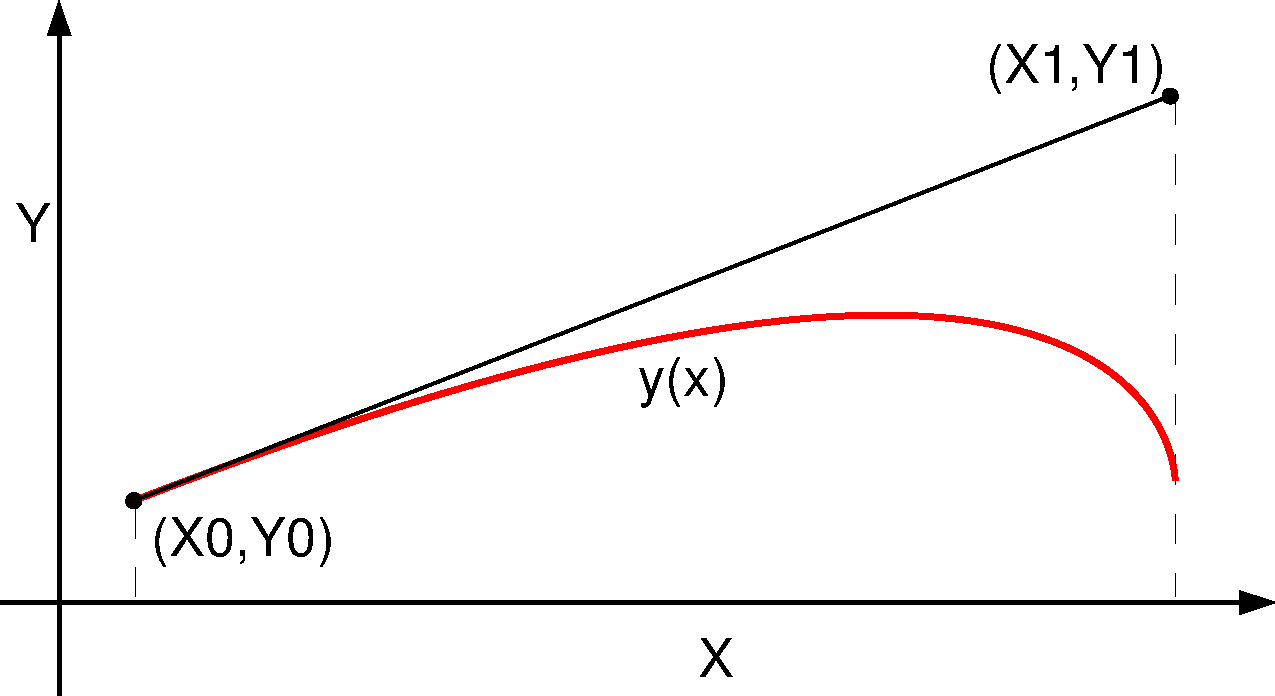
\includegraphics[width=10cm,keepaspectratio]{picture/eulero}
		\centering
		\label{fig:eulero}

	\end {minipage}
		\quad
	\begin{minipage}{.30\textwidth}
		\caption{Metodo di Eulero}
		\begin{equation}
		y_{1}=y_{0} + h F(x_{0},y_{0})
		\end{equation}
	\end {minipage}%
	}

\end{figure}

Dalla definizione è evidente la sua relazione con gli algoritmi di Runge-Kutta, non è altro che il metodo di ordine 1, dove i parametri $\alpha$ e $\theta$ non entrano ancora in gioco ( per questo il metodo di primo ordine è unico) e il parametro di peso è unitario visto che per ogni intervallo di campionamento il punto utilizzato per calcolare l'approssimazione dello step successivo è solo uno.

\subsection{Metodo del Correttore}
Consiste sostanzialmente in un affinamento del metodo precedente.

Per stimare la soluzione nel punto $x_{0}+h$ non viene utilizzato il valore della derivata nel punto $x_{0}$, che viene fornita attraverso la funzione $f(x,y)$ dell'equazione differenziale,  ma viene utilizzata nella formula del incremento finito una stima del valore della derivata nel punto medio dell'intervallo.

	\begin{equation}
	y_{1}=y_{0} + h F(x'_{0},y'_{0})
	\end{equation}

dove  $x'_{0}=x_{0} + \frac{h}{2}$ e $y'_{0} = y_{0} + \frac{h}{2}F(x_{0},y_{0})$.

\begin{figure}[!h]
\caption{Metodo del Correttore}
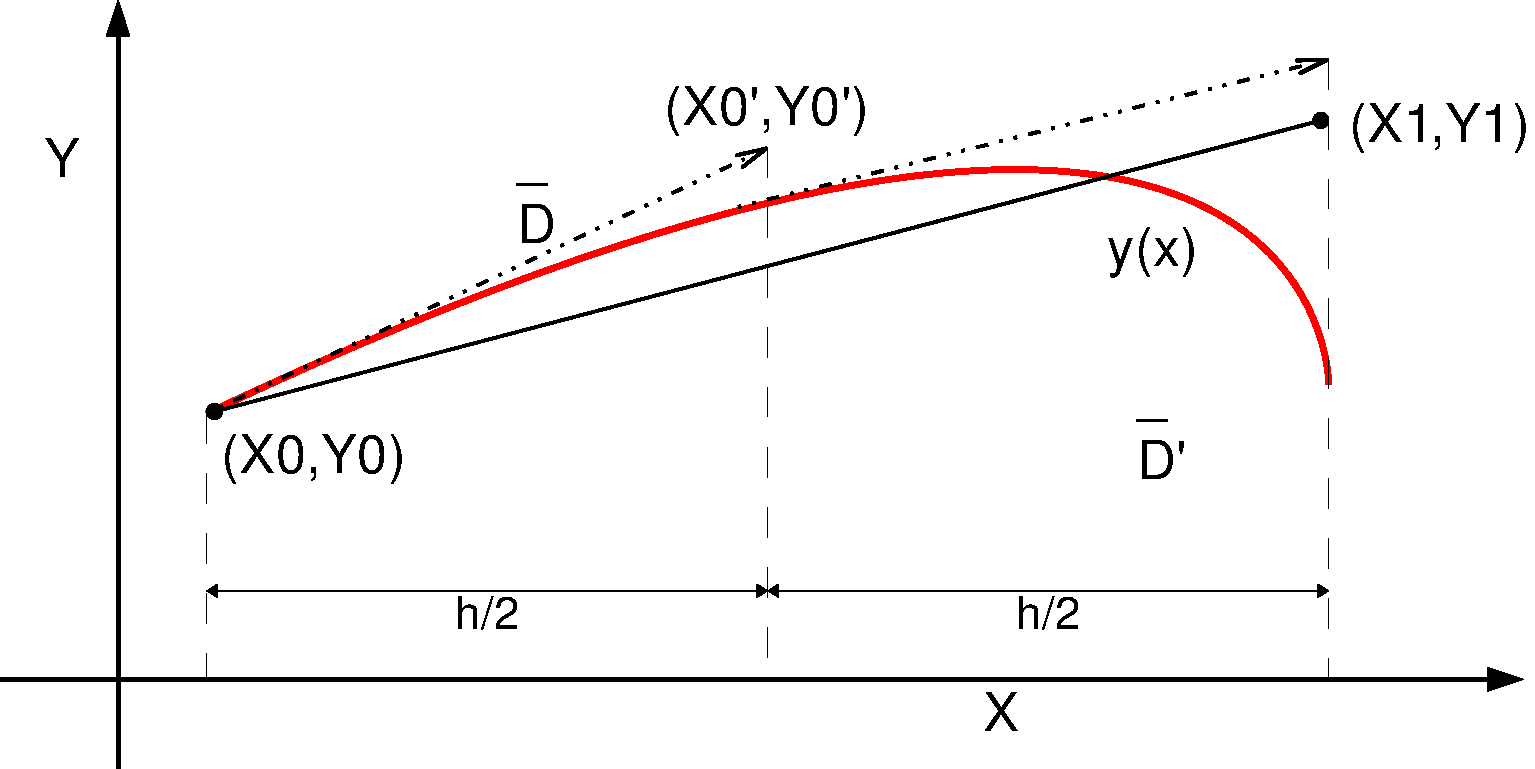
\includegraphics[width=10cm,keepaspectratio]{picture/correttore}
\centering
\label{fig:correttore}
\end{figure}

La ragione di questo nome è nel fatto che il valore della funzione dopo l'incremento $h$ non viene stimata con la derivata nel punto iniziale ma viene preso una correzione di tale valore, la derivata nel punto medio.

Anche questo metodo fa parte della classe dei metodi R-K, l'ordine è 2 per stimare il punto destro dell'intervallo vengono presi 2 punti all'interno, il primo è l'estremo sinistro con peso nullo e il secondo è il punto medio con peso unitario.
I parametri nella formula di R-K generico (6) sono $ (\omega_{0}=0)$ e $(\omega_{1}=1 , \theta_{1}=\frac{1}{2}, \alpha_{1}=f(x_{0},y_{0}))$

\subsection{Runge Kutta di quarto ordine}

Esistono diversi metodi di integrazione che stimano la soluzione del problema (1) in un punto valutando la funzione $f$ in 4 punti dell'intervallo precedente,  l'algoritmo utilizzato usualmente è il seguente:

\begin{displaymath}
	\begin{array}{rcl}
				K_{0} & = & h f(x_{0} , y_{0}) \\
				K_{1} & = & h f(x_{0} + h/2 , y_{0} + K_{0}/2) \\
				K_{2} & = & h f(x_{0} + h/2 , y_{0} + K_{1}/2) \\
				K_{3} & = & h f(x_{0} + h , y_{0} + K_{2}) \\
	\end{array}
\end{displaymath}

	\begin{equation}
	y_{1} = y_{0} + ( K_{0} + 2 K_{1} + 2 K_{2} + K_{3})/6
	\end{equation}
  
Dalla definizione è evidente la sua parentela con l'idea fondamentale dell'incremento finito. 

Ad ogni step dell' algoritmo la funzione $f(x,y)$, in altre parole la derivata prima, viene stimata in quattro punti, una volta all'inizio, due volte nel mezzo e una volta nell'estremo destro del'intervallo dell'ascissa. 

Alla fine l'incremento finito della soluzione dopo lo step di ampiezza $h$ viene approssimato mediando in modo pesato le 4 derivate prime calcolate.

\begin{figure}[!h]
\caption{Metodo Runge Kutta : progressione dei punti valutati al IV ordine}
\
includegraphics[width=8cm,height= 4cm]{picture/runge}
\centering
\label{fig:correttore}
\end{figure}

Come tutti gli altri metodi R-K è discreto, iterativo e a singolo passo ma ha la proprietà aggiuntiva di avere una struttura particolarmente semplice: i termini $K_{n}$ sono calcolati in successione, l'n-simo coefficiente dipende unicamente dall' (n-1)-simo. Questi algoritmi possono generalizzarsi all'ordine $n$ nella forma:

\begin{displaymath}
	\begin{array}{rcl}
				K_{0} & = & h f(x_{0} , y_{0}) \\
				K_{1} & = & h f(x_{0} + \theta_{1} h , y_{0} + \theta_{1} K_{0}) \\
				\vdots \\
				K_{n} & = & h f(x_{0} + \theta_{n} h , y_{0} + \theta_{n} K_{n-1}) \\
	\end{array}
\end{displaymath}

	\begin{equation}
	y_{1} = y_{0} + \sum_{j=0}^{\nu}\omega_{j}K_{j}
	\end{equation}

Convenzionalmente ci si riferisce a questo algoritmo come "Runge-Kutta di quarto ordine".
 
\subsection{Ordine di Correttezza degli algoritmi}
Come detto precedentemente, per ordine di un algoritmo di integrazione di O.D.E. si intende fino a che ordine dello sviluppo di taylor la soluzione approssimata ricalca la soluzione attesa.
\begin{figure}[!htbp]
	\caption{Rappresentazione grafica della dispersione tra valore numerico e valore atteso}
	\centering
	\subfigure{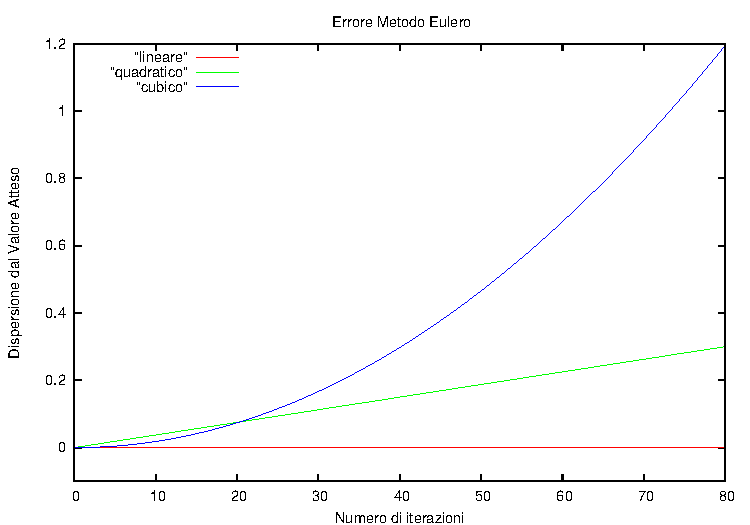
\includegraphics[width=13cm,height=7cm]{picture/eul}}\\

 	\subfigure   {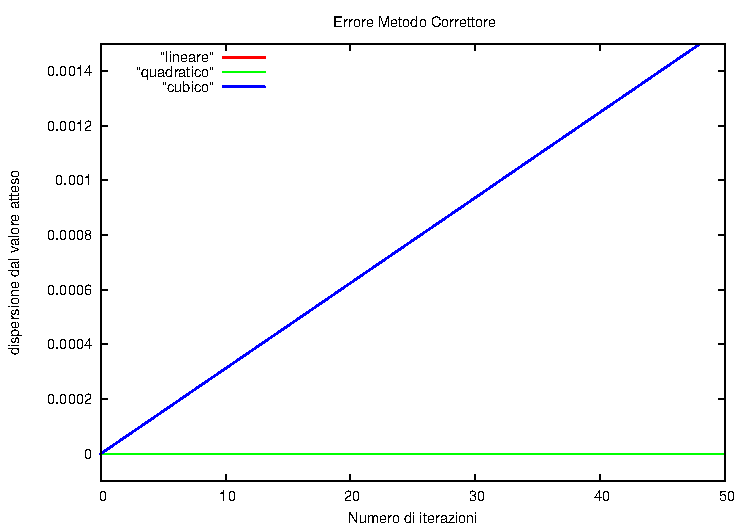
\includegraphics[width=13cm,height=7cm]{picture/cor}}\\

	\subfigure   {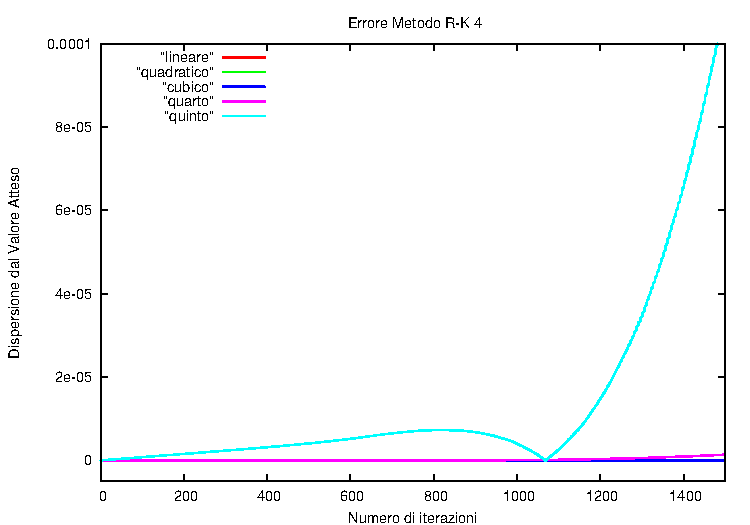
\includegraphics[width=13cm,height=7cm]{picture/kut}}\\
		\label{fig:tau}
\end{figure}
Un possibile modo per stimare questo fattore è quello di integrare numericamente problemi di cauchy del tipo:
\begin{equation}
	\left\{ 
			\begin{array}{rcl}
 			\dot{y(t)} &=& \alpha x^{n-1}\\
 			y(t_{0}) &=& y_{0} \\
  			\end{array} \right.
	\end{equation}
la soluzione di questa equazione è una potenza ennesima di x, $y=\dfrac{\alpha x^{n}}{n}+y_{0}$.

A questo punto stampando per ogni metodo, al crescere delle iterazioni, il valore assoluto della differenza fra valore ottenuto e valore atteso di queste funzioni semplici, si ottiene una stima grafica dell'andamento dell'incertezza del n-simo termine di un polinomio.

In questo modo si può ottenere una visualizzazione grafica ( \ref{fig:tau}), non rigorosa ma indicativa, del termine di correttezza dello sviluppo della soluzione.

Come si vede dai grafici \ref{fig:tau}, l'errore cresce al crescere dei punti stimati, questo è inevitabile e consegue dalla propagazione dell'errore.
Apparentemente l'andamento della crescita è una potenza del ordine del termine meno quello dello del metodo.

La natura progressiva del metodo, che stima un punto basandosi esclusivamente sulle informazioni della soluzione nel punto precedente, fa si che l'incertezza di ciascun punto risenta non solo della precisione del metodo ma anche del errore sul valore della soluzione nel punto precedente.
Ovviamente ridurre il numero dei punti non aggira il problema, la validità dei metodi di integrazione si fonda sulla possibilità di approssimare una funzione con il suo sviluppo polinomiale troncato e questo è analiticamente ragionevole solo per intervalli sulle ascisse "piccoli".

In queste simulazioni è stato usato un incremento di $\tau = 0,05$, i grafici per uno step più piccolo risulterebbero identici ma scalati su errori assoluti minori.
In conclusione l'ordine di approssimazione di $\tau$ degli algoritmi risulta:
    			
\begin{displaymath}
\centering
\begin{array}{|c|c|}
\hline
metodo & errore \\
\hline
\hline
EULERO &  o(\tau) \\
\hline
CORRETTORE &  o(\tau^2) \\
\hline
R-K 4 &  o(\tau^4) \\
\hline
\end{array}
\end{displaymath}


Il metodo "Runge-Kutta 4" risulta fra tutti il più preciso, ma bisogna ricordare che l'errore che ogni algoritmo può presentare nella stima della n-simo punto della soluzione non dipende solo da esso ma anche dal punto, l'incertezza cresce con il numero di iterazioni.
\clearpage

\subsection{Estensione dei metodi R-K ad O.D.E. di ordine superiore al primo}
Si consideri il problema di Cauchy di grado n:
	\begin{equation}
	\left\{ 
			\begin{array}{lcl}
 			\dot{x}^{(n)} &=& F(t , x , x', \ldots ,x^{(n-1)})\\
 			x(t_{0}) &=& x_{0} \\
			\dot{x}(t_{0}) &=& \dot{x}_{0} \\
			 & \vdots & \\
			x^{(n-1)}(t_{0}) &=& x^{(n-1)}_{0} \\
  			\end{array} \right.
	\end{equation}
Con il cambio di coordinate stadard $ x^{(j)}(t) = Z_{j+1}(t) $ si può trasformare un'equazione differenziale ordinaria di ordine n in un sistema di n equazioni ordinarie di primo ordine.

	\begin{displaymath}
	\left\{ 
			\begin{array}{lcl}
 			\dot{Z}_{1} &=& Z_{2}\\
 			\dot{Z}_{2} &=& Z_{3}\\
			 & \vdots & \\
			\dot{Z}_{n-1} &=& Z_{n}\\
			\dot{Z}_{n} &=& F(t , Z_{1} , \ldots , Z_{n})\\
			\end{array} \right.
	\end{displaymath}

Introducendo la notazione vettoriale a n componenti dove la prima colonna del sistema precedente è la derivata prima del vettore $(Z_{1}(t) ,\ldots, Z_{n}(t))$ mentre la seconda è la rappresentazione in componenti di una funzione $ G(t,\vec{Z}) : R^{n+1} \longrightarrow R^{n}$ 

si ottiene il problema : 
	\begin{equation}
	\left\{ 
			\begin{array}{lcl}
 			\dot{\vec{Z}} &=& G(t, \vec{Z})\\
 			\vec{Z}(t_{0}) &=& \vec{x_{0}} \\
  			\end{array} \right.
	\end{equation}

Che non è altro che un problema di Cauchy di primo ordine con una funzione soluzione di n componenti.
$\vec{Z}(t_{0})$ è il vettore dei termini noti del problema di ordine n tradotto nella notazione con le funzioni $Z_{i}$.

L'estensione di qualsiasi metodo R-K ad equazioni differenziali di grado superiore al primo è simbolicamente ovvio. La forma più generale possibile sarà:
\begin{displaymath}
	\begin{array}{rcl}
				\vec{K}_{0} & = & h G(t_{0} , \vec{Z}(t_{0})) \\
				\vec{K}_{1} & = & h G(t_{0} + \theta_{1} h , \vec{Z}(t_{0}) + \theta_{1} \alpha_{1}) \\
				\vdots \\
				\vec{K}_{n} & = & h G(t_{0} + \theta_{n} h ,\vec{Z}(t_{0}) + \theta_{n} \alpha_{n}) \\
	\end{array}
\end{displaymath}

	\begin{equation}
	\vec{Z}' = \vec{Z}_{0} + \sum_{j=0}^{\nu}\omega_{j}\vec{K}_{j}
	\end{equation}

Rendendosi conto che $G(t, \vec{V})$ è semplicemente un operatore che scala di un posto verso l'alto gli elementi del vettore $\vec{V}$ e pone come ultima componente il valore della funzione $F(t, \vec{V})$ e limitandosi al caso semplice dei metodi R-K del tipo (10), dove il coefficiente $K_{n}$ è dipende esclusivamente dal coefficiente $K_{n-1}$ direttamente precedente, si trova la forma esplicità dei termini $K$.

	\begin{equation}
	\vec{K_{0}} = h \left[ 
				\begin{array}{c}
 				Z_{2}(t_{0}) \\
				\vdots \\
				Z_{n}(t_{0}) \\
 				F(t_{0} , \, Z_{1}(t_{0}) , \ldots ,\, Z_{n}(t_{0}) )  \\
  				\end{array} \right]
\qquad
	\vec{K_{n}} = h \left[ 
				\begin{array}{c}
 				(\vec{Z}(t_{0}) + \theta_{n}\vec{K}_{n-1})_{2} \\
				\vdots \\
				(\vec{Z}(t_{0}) + \theta_{n}\vec{K}_{n-1})_{n}\\
 				F(t_{0} + \theta_{n} h,\, \vec{Z}(t_{0}) + \theta_{n}\vec{K}_{n-1} )  \\
  				\end{array} \right]
	\end{equation} 


Questa non è l'unica possibile estensione a più variabile dei metodi R-K.

Si consideri per semplicità un generico sistema di due equazioni differenziali ordinarie di primo ordine:
	\begin{equation}
	\left\{ 
			\begin{array}{rcl}
 			\dot{x(t)} &=& F(t, x(t), u(t))\\
			\dot{u(t)} &=& G(t, x(t), u(t)) \\
			\end{array} \right.
	\end{equation}
con valori iniziali all'istante iniziale $t_{n}$ fissati: $x_{n} = x(t_{n})$ e $u_{n} = u(t_{n})$.

A questo punto si può pensare di applicare naturalmente l'algoritmo R-K4 ad ogni equazione differenziale del sistema presa singolarmente. Ovverro si calcolano:

	\begin{equation}\begin{array}{rcl}
	x_{n+1} &=& x_{n} + (k_{0} + 2 k_{1} + 2 k_{2} + k_{3})/6\\
	u_{n+1} &=& u_{n} + (m_{0} + 2 m_{1} + 2 m_{2} + m_{3})/6\\
	\end{array}\end{equation}

Dove:
\begin{displaymath}
	\begin{array}{rcl}
				k_{0} & = & h F(t_{n} , x_{n} , u_{n}) \\
				k_{1} & = & h F(t_{n} + h/2 , x_{n} + k_{0}/2 , u_{n} + m_{0}/2) \\
				k_{2} & = & h F(t_{n} + h/2 , x_{n} + k_{1}/2, u_{n} + m_{1}/2) \\
				k_{3} & = & h F(t_{n} + h , x_{n} + k_{2}, u_{n} + m_{2}) \\
	\end{array} \qquad
	\begin{array}{rcl}
				m_{0} & = & h G(t_{n} , x_{n} , u_{n}) \\
				m_{1} & = & h G(t_{n} + h/2 , x_{n} + k_{0}/2 , u_{n} + m_{0}/2) \\
				m_{2} & = & h G(t_{n} + h/2 , x_{n} + k_{1}/2, u_{n} + m_{1}/2) \\
				m_{3} & = & h G(t_{n} + h , x_{n} + k_{2}, u_{n} + m_{2}) \\
	\end{array}
\end{displaymath}

Questa formulazione è un estensione abbastanza intuitiva del algoritmo fatto per una singola variabile, il primo passo è il calcolo della derivata prima di $x$ e di $u$ nel punto iniziale $t_{0}$, da queste si calcolano $k_{0}$ e $m_{0}$ che sono una prima stima dell'incremento finito delle due soluzioni $x(t)$ e $u(t)$ dopo lo step $h$.

Questi due coefficienti vengono poi utilizzati per ottenere una prima stima delle derivate delle soluzioni (passando chiaramente attraverso le funzioni $F$ e $G$) nel punto medio e così via esattamente come si è costruito il metodo per l'equazione singola.

In modo analogo a quanto fatto prima è possibile vedere un equazione differenziale di secondo grado come un sistema di 2 equazioni, definendo $\dot(x)(t) = u(t)$, basterà porre nel sistema di equazioni (11) $F(t, x(t), u(t)) =u(t)$ per ottenere l'algoritmo corrispondente a questo tipo di problemi.
A questo punto l'implementazione in \emph{C++} è praticamente ovvia:

\begin{lstlisting}[frame=single]
void RK4(double (*G)(double,double,double), double *p0,double h) //ingresso: funzione, valori iniziali, incremento
{
	double x=p0[0];
	double y=p0[1];
	double u=p0[2];
	double k[4],m[4];

	k[0] = h * u;
	m[0] = h * G(x,y,u) ;
	k[1] = h * (u+ m[0]/2);
	m[1] = h * G(x + h/2 , y +k[0]/2 , u +m[0]/2);
	k[2] = h * (u+ m[1]/2);
	m[2] = h * G(x + h/2, y + k[1]/2 , u + m[1]/2);
	k[3] = h * (u + m[2]);
	m[3] = h * G(x+h,y + k[2], u + m[2]);
	
	p0[0] = x +h;
	p0[1] = y + (k[0]+2*k[1]+2*k[2]+k[3])/6;
	p0[2] = u + ( m[0] + 2*m[1] + 2*m[2] +m[3])/6;
}
\end{lstlisting}

\section{Casestudy}
\paragraph{Pendolo Caotico}
E' il sistema fisico formato da un pendolo rigido, di lunghezza $R$ e massa $M$, vincolato a muoversi su un piano verticale (rotatore rigido piano) su cui incidono 3 forze:
\begin{itemize}
	\item[-] Forza peso: modulo $ F_{g} = mg$, direzione verticale.
	\item[-] Forza d'attrito : $ \vec{F}_{\eta} = - \eta \vec{v}$, stessa direzione ma verso opposto alla velocità e di modulo proporzionale ad un parametro $\eta$.
	\item[-] Forzante armonica: la direzione ruota con velocità angolare fissa $\omega$ mentre il modulo $ F_{c} = F_{0}$ è costante.
	\end{itemize}
Come si può vedere nella figura \ref{fig:pendu}.
 
\begin{figure}[!h]
\centering
\mbox{%
		\begin{minipage}{.30\textwidth}
			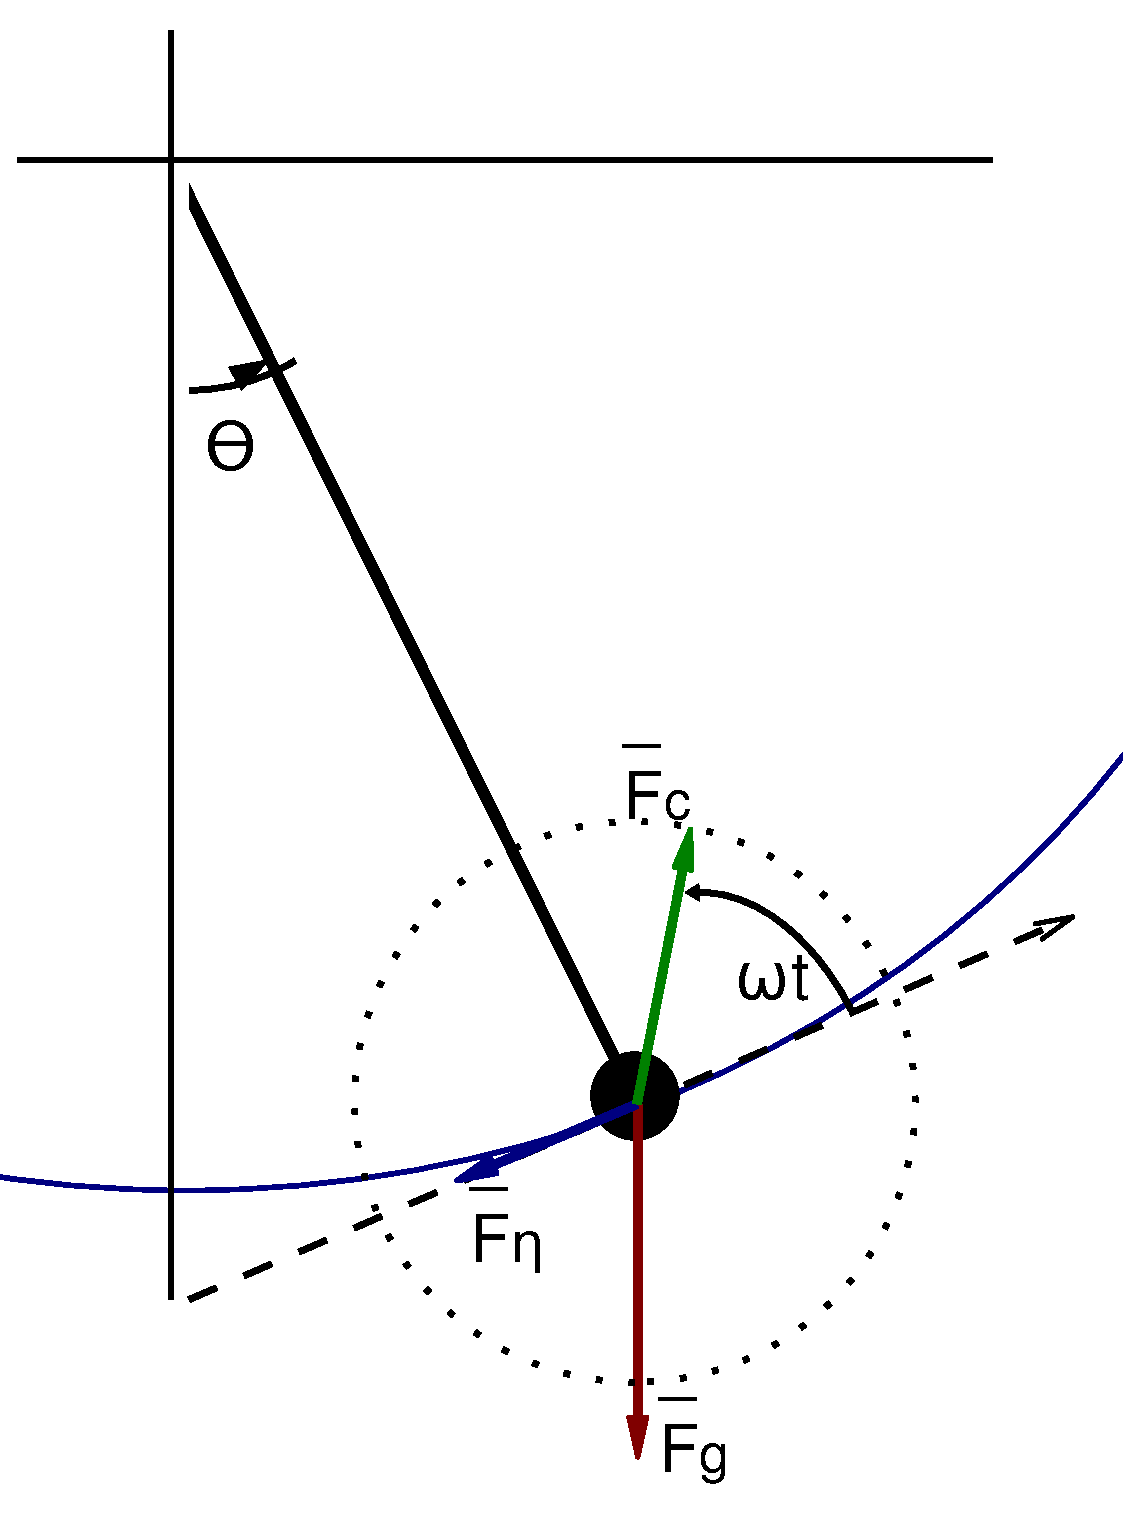
\includegraphics[width=\textwidth,keepaspectratio]{picture/pendu}
		\label{fig:pendu}
		\end {minipage}
		\quad
		\begin{minipage}{.30\textwidth}
		\caption{Modello di Pendolo Caotico}
		\end {minipage}%
	}

\end{figure}

\paragraph{equazioni del moto}
Il sistema ha solo un grado di libertà, scegliendo come coordinata di configurazione l'angolo $\theta$ sotteso dalla verticale e dalla direzione del rotatore, si ricava l'equazione di newton del sistema:
	\begin{equation}\begin{array}{rcl}
	I\, \ddot{\theta} &=& \sum \tau \qquad = \\
	=\,\, m\, R^{2}\, \ddot{\theta} &=& R( F_{0}\cos(\omega t) -m g \sin(\theta) -\eta R \dot{\theta})\\
	\end{array}\end{equation}

che conduce alla seguente O.D.E. di secondo grado
	\begin{equation}
\ddot{\theta} \, = \, \dfrac{F_{0}}{mR}\cos(\omega t) - \dfrac{g}{R}\sin(\theta) -\eta R \dot{\theta}
	\end{equation}

Scegliendo per semplicità un pendolo di massa 1 $kg$ e lunghezza 9,8 $m$ (in altre parole la costante moltiplicativa $B=\frac{g}{R}$ del seno viene fissata ad $ 1 s^{-2}$) rimangono da fissare a seconda dei casi le costanti che definiscono la struttura del sistema
	\begin{displaymath}
	A= \dfrac{\eta}{m} \qquad \Phi = \dfrac{F_{0}}{mR} \qquad \omega  
	\end{displaymath}
e le condizioni al iniziali $\theta (t_{0})$ e $\dot{\theta}(t_{0})$.


\clearpage
\section{Risultati}

\subsection{Applicazione R-K4 a casi banali}
Studo della dinamica del sistema risolvendo numericamente l'equazione del moto.
\begin{figure}[!h]
\caption{}
\paragraph{Pendolo semplice}

Dati: $A$ = 0 ; $\Phi$ = 0 ; $\theta(t_{0}) = \pi /4$ 
\centering
\subfigure[legge oraria]{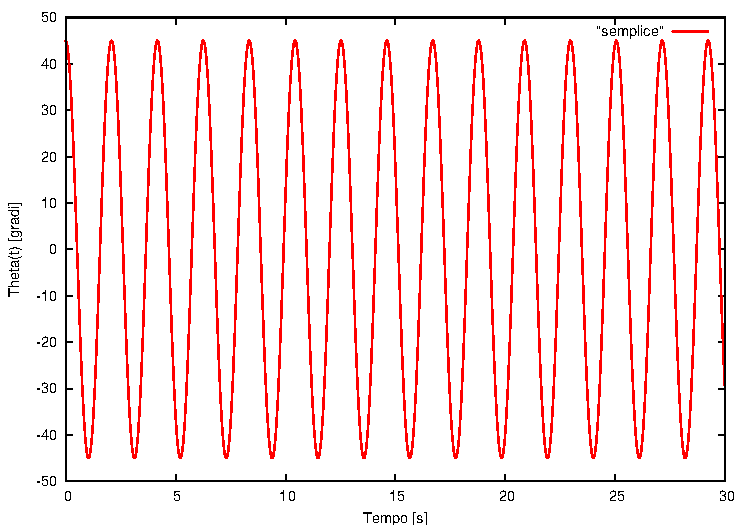
\includegraphics[width=9cm,keepaspectratio]{picture/semplice}}\,
\subfigure[spazio fasi]{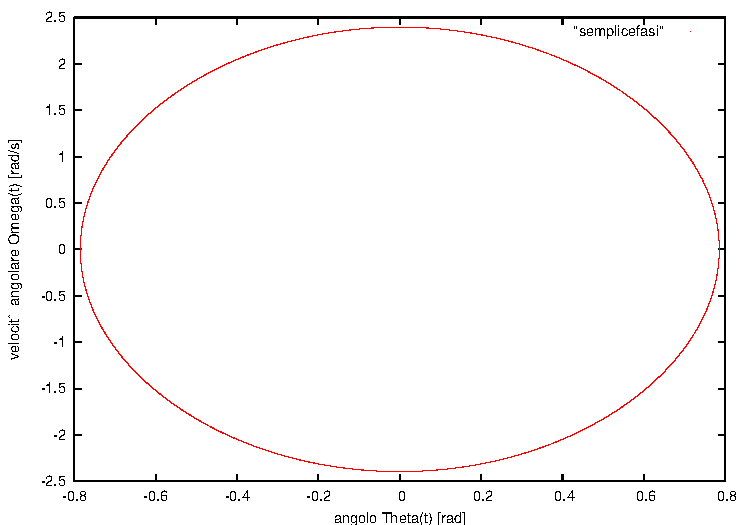
\includegraphics[width=9cm,keepaspectratio]{picture/semplicefasi}}
\end{figure}

\begin{figure}[!h]
\caption{}
\paragraph{Pendolo smorzato}

Dati: $A = 0,25 \, s^{-1}$ ; $\Phi$ = 0 ; $\theta(t_{0}) = \pi /4$ 
\centering
\subfigure[legge oraria]{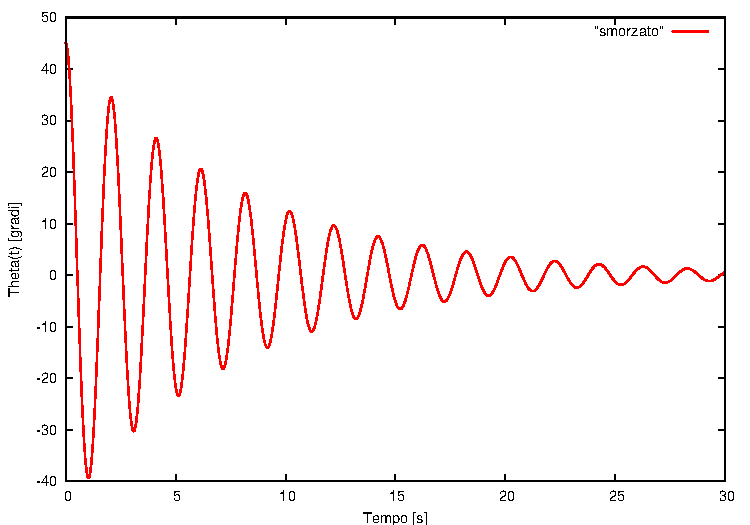
\includegraphics[width=14cm,keepaspectratio]{picture/smorzato}}\,
\subfigure[spazio fasi]{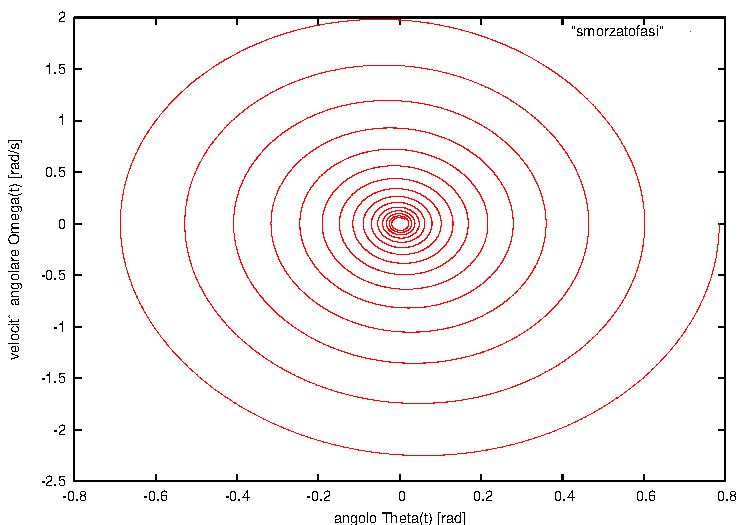
\includegraphics[width=14cm,keepaspectratio]{picture/smorzatofasi}}
\end{figure}
 
\begin{figure}[!h]
\caption{}
\paragraph{Pendolo Forzato}

Dati: $A$ = 0 ; $\Phi = 1,5 \, s^{-2} $ ; $\omega = 0,66 \, s^{-1}$ ; $\theta(t_{0}) = \pi /4$
\centering
\subfigure[legge oraria]{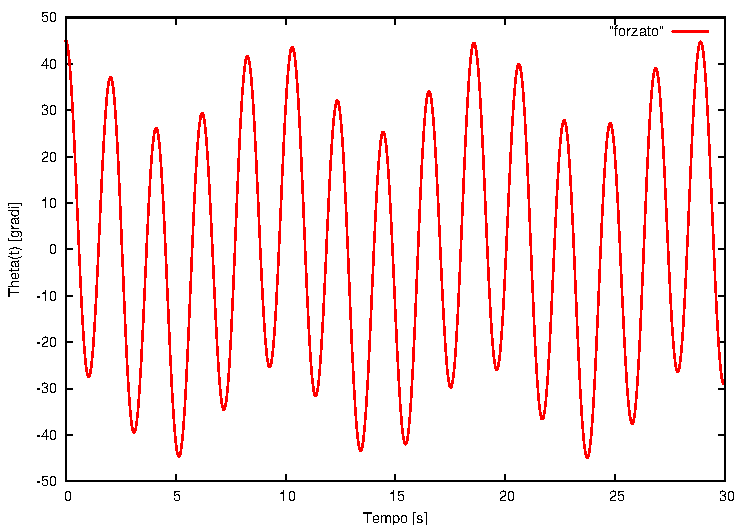
\includegraphics[width=14cm,keepaspectratio]{picture/forzato}}\,
\subfigure[spazio fasi]{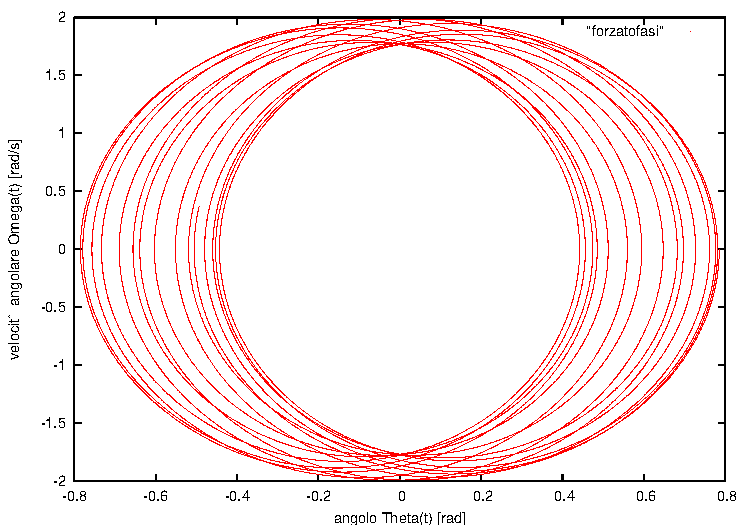
\includegraphics[width=14cm,keepaspectratio]{picture/forzatofasi}}
\end{figure}

\begin{figure}[!h]
\caption{}
\paragraph{Pendolo Caotico}

Dati: $A = 0,25 \, s^{-1}$ ; $\Phi = 1,5 \, s^{-2} $ ; $\omega = 0,66 \, s^{-1}$ ; $\theta(t_{0}) = \pi /4$ 
\centering
\subfigure[legge oraria]{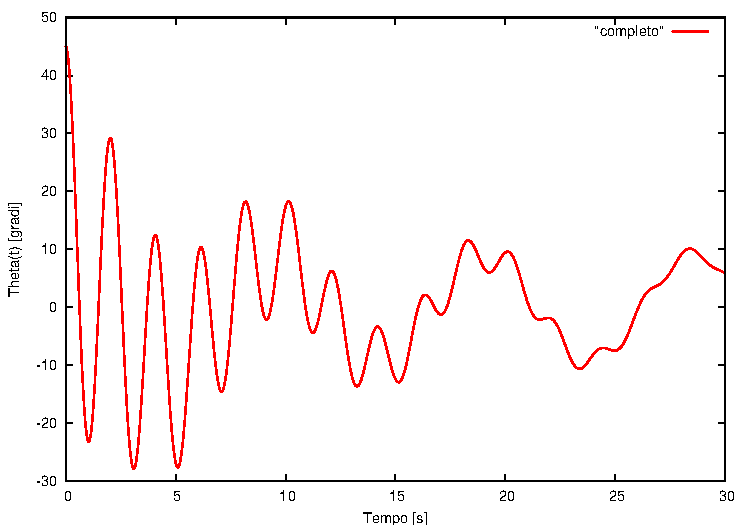
\includegraphics[width=14cm,keepaspectratio]{picture/completo}}\,
\subfigure[spazio fasi]{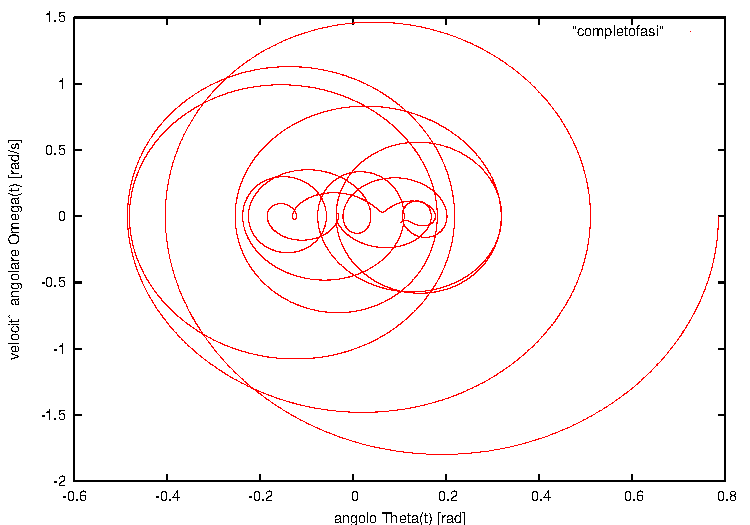
\includegraphics[width=14cm,keepaspectratio]{picture/completofasi}}
\end{figure}

\clearpage
\subsection{Caoticità del Sistema}
Conoscendo esattamente l'equazioni del moto l'evoluzione del sistema è perfettamente deterministica. Nonostante questa c'è forte dipedenza del evoluzione del sistema dai parametri iniziali, in altre parole una variazione infinitesima dei coefficienti strutturali ($\eta$ , $\Phi$ , $\omega$ , $\theta_{0}$) del sistema attorno a particolari valori critici determinano una notevole divergenza tra le due traiettorie corrispondenti alle diverse configurazioni.

Questo fenomeno è detto Pseudo-Caoticità del sistema: due istanze di un sistema che partono con condizioni inizali molto simili si separano molto rapidamente, l'evoluzione dipende molto sensibilmente dalle condizioni iniziali.

\paragraph{Individuazione delle configurazioni caotiche}

La prima cosa che si può dimostrare sperimentalmente è che il sistema non ha comportamento caotico per ogni configurazione.
Si studiano numericamente le traiettorie del sistema in 3 configurazioni che differiscono solo per il valore del parametro $\Phi$.

Parametri comuni:
\begin{displaymath}
\begin{array}{|c|c| |c|c|}
\hline
A = 0,5 &  \omega = 0,66 s^{-1} & \theta_{0} = 0 & dot{\theta}_{0} = 0\\
\hline
\end{array}
\end{displaymath}

Parametri variati:
\begin{displaymath}
\begin{array}{|c|c|}
\hline
F0\_\textrm{alta} &  \Phi = 2,150 \, s^{-2}\\
\hline
F0\_\textrm{caos} &  \Phi = 1,48555\, s^{-2}\\
\hline
F0\_\textrm{bassa} &  \Phi = 0,150 \, s^{-2}\\
\hline
\end{array}
\end{displaymath}

Nella figura \ref{fig:individuazconfronto} è possibile vedere a confronto le tre traiettorie, nel grafico è evidente la peridiocità delle due configurazioni limite a dispetto della apparente casualità della soluzione intermedia, ci si aspetterà che i parametri della configurazione F0\_\textrm{caos} siano nell'intorno della configurazione caotica.

Nelle figure \ref{fig:individuazalta} e \ref{fig:individuazbassa} si prende invece in esame il comportamento delle configurazioni estreme per piccole variazioni del parametro $\Phi$. 

Si nota subito che nell'intorno di questi valori le traiettorie variano in modo continuo per piccole variazioni ($\pm 0,005 \, s^{-2}$) del parametro A.

In queste configurazioni il sistema non mostra quindi un coportamento pseudo-caotico, sono in un certo senso in equilibrio stabile vicino alle configurazioni $F0\_\textrm{alta} $ e $F0\_\textrm{bassa} $.

(oss: per tutti i grafici relativi agli spazi delle fasi è stato trascurato il transiente iniziale)

\paragraph{Illustazione del comportamento caotico}

Individuata approssimativamente la regione di "instabilità" delle soluzione attorno ai parametri di F0\_caos si può mostrare il senso della pseudocaoticità costruendo il grafico di altri 2 sistemi i cui parametri differiscono infinitesimamente dal soluzione caotica: grafici \ref{fig:caostheta} , \ref{fig:caosforz} e \ref{fig:caosomega}.
I sistemi che si trovano in questa regione di parametri avranno una traiettoria che dopo un tempo finito biforcherà da quella infinitesimamente vicina.

\begin{figure}[!h]
\caption{}
\label{fig:individuazconfronto}
\paragraph{Confronto dei 3 pendoli con diverse forzanti}
\label{fig:individuazconfronto}
\centering
\subfigure[Traiettorie]{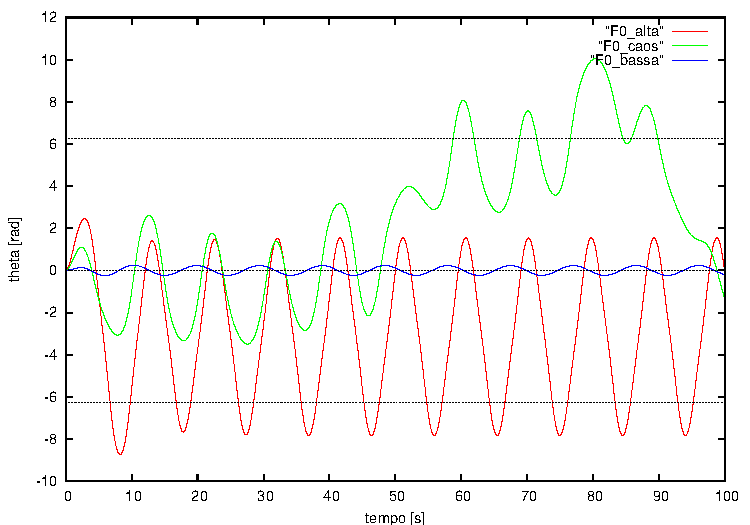
\includegraphics[width=13.5cm,keepaspectratio]{picture/individuazione/confrontoF0}}\,
\subfigure[Spazio delle Fasi]{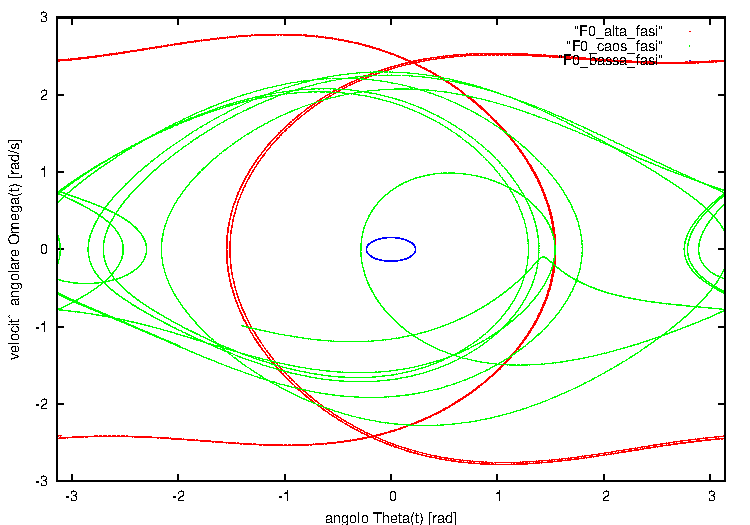
\includegraphics[width=13.5cm,keepaspectratio]{picture/individuazione/confrontoF0_fasi}}
\end{figure}

\begin{figure}[!h]
\caption{}

\paragraph{Confronto fra 3 configurazioni intorno ad F0\_alta}
\label{fig:individuazalta}
\centering
\subfigure[Traiettorie]{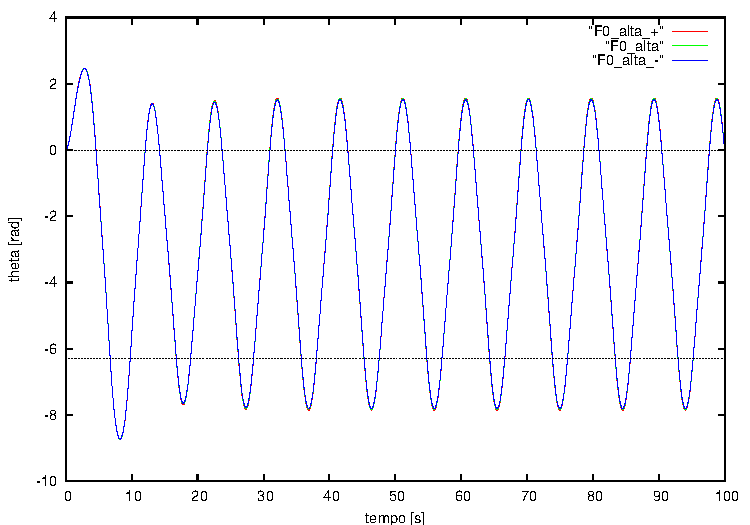
\includegraphics[width=13.5cm,keepaspectratio]{picture/individuazione/F0_alta}}\,
\subfigure[Spazio delle Fasi]{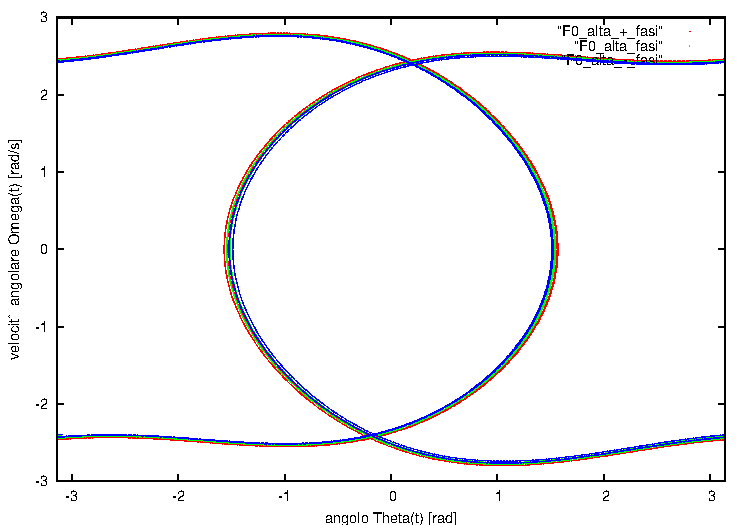
\includegraphics[width=13.5cm,keepaspectratio]{picture/individuazione/F0_alta_fasi}}
\end{figure}

\begin{figure}[!h]
\caption{}
\paragraph{Confronto fra 3 configurazioni intorno ad F0\_bassa}
\label{fig:individuazbassa}
\centering
\subfigure[Traiettorie]{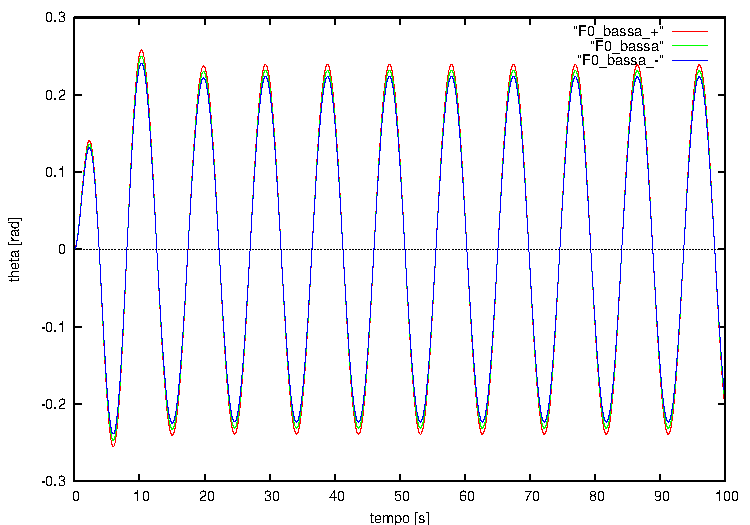
\includegraphics[width=13.5cm,keepaspectratio]{picture/individuazione/F0_bassa}}\,
\subfigure[Spazio delle Fasi]{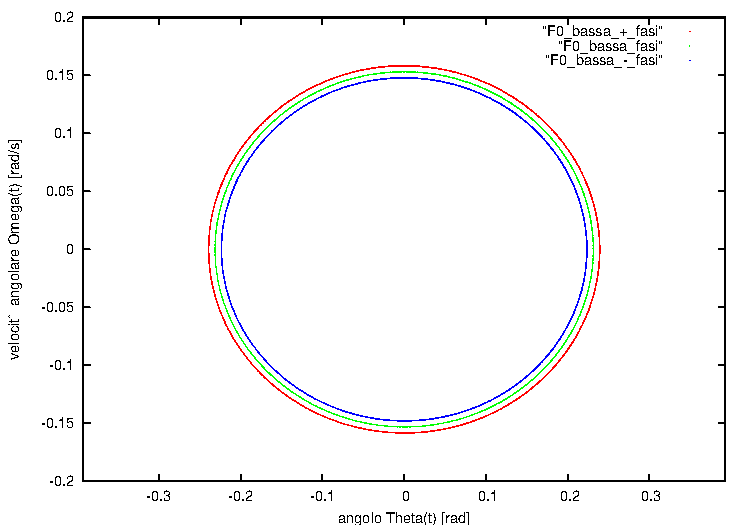
\includegraphics[width=13.5cm,keepaspectratio]{picture/individuazione/F0_bassa_fasi}}
\end{figure}

\clearpage


\begin{figure}[!h]
\caption{}
\paragraph{3 traiettorie di pendolo con angolo iniziale $\theta$ variato di $\pm$0.005 rad attorno ad  F0\_caos}
\label{fig:caostheta}
\centering
\subfigure[Traiettorie]{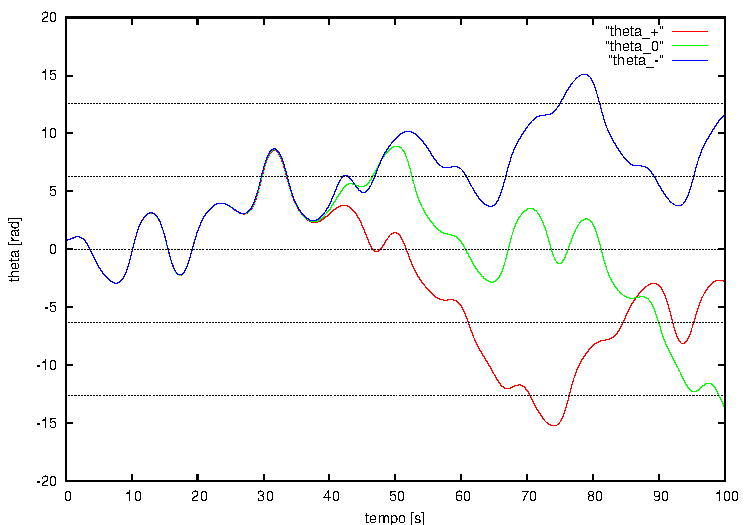
\includegraphics[width=13.5cm,keepaspectratio]{picture/chaos/confrontotheta}}\,
\subfigure[Spazio delle Fasi]{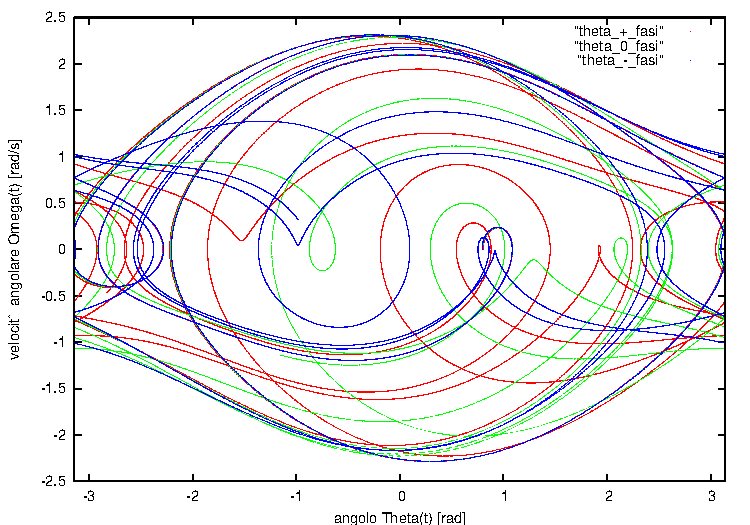
\includegraphics[width=13.5cm,keepaspectratio]{picture/chaos/confrontotheta_fasi}}
\end{figure}

\begin{figure}[!h]
\caption{}
\paragraph{traiettorie di 3 pendoli con forzanti  variate di  $\pm0.005 \, s^{-2}$ rispetto al valore di F0\_caos}
\label{fig:caosforz}
\centering
\subfigure[Traiettorie]{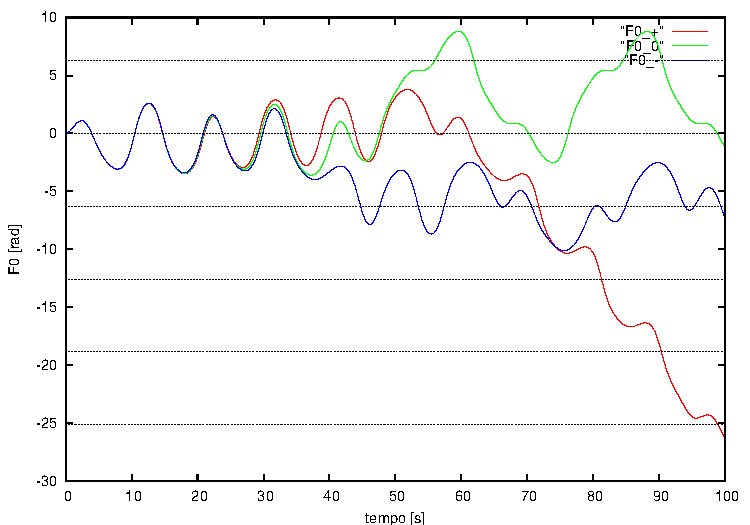
\includegraphics[width=13.5cm,keepaspectratio]{picture/chaos/confrontoF0}}\,
\subfigure[Spazio delle Fasi]{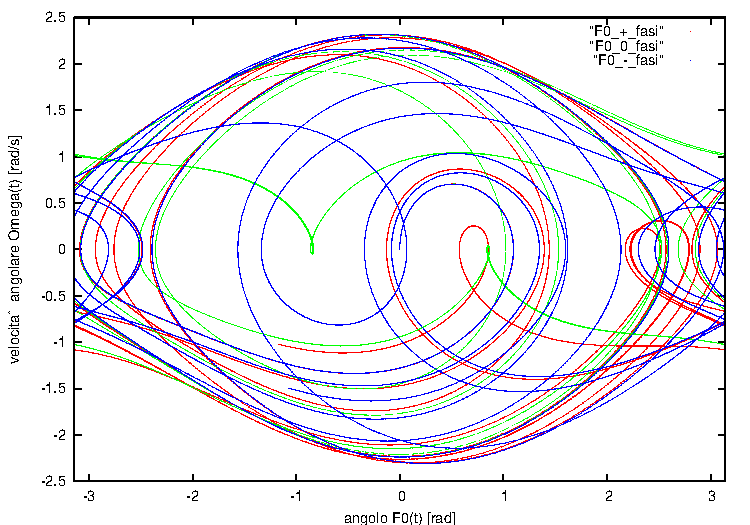
\includegraphics[width=13.5cm,keepaspectratio]{picture/chaos/confrontoF0_fasi}}
\end{figure}

\begin{figure}[!h]
\caption{}
\paragraph{traiettorie di 3 pendoli con frequenza delle forzanti  variate di $\pm0.00005 \, s^{-2}$ rispetto al valore di F0\_caos}
\label{fig:caosomega}
\centering
\subfigure[Traiettorie]{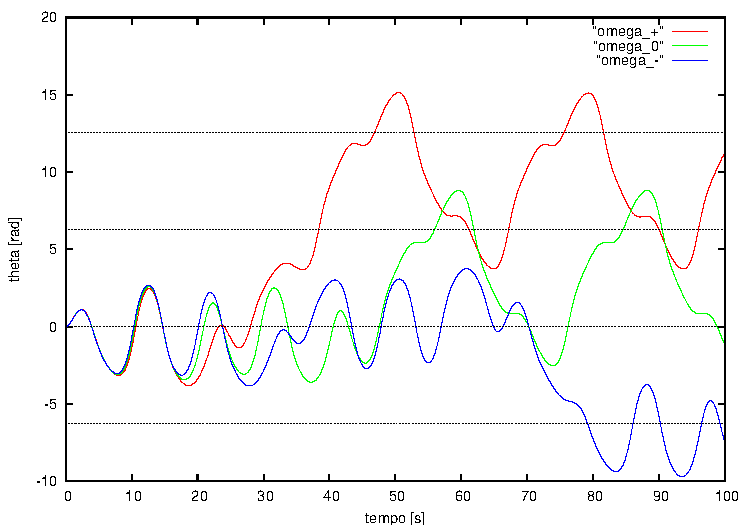
\includegraphics[width=13.5cm,keepaspectratio]{picture/chaos/confrontoomega}}\,
\subfigure[Spazio delle Fasi]{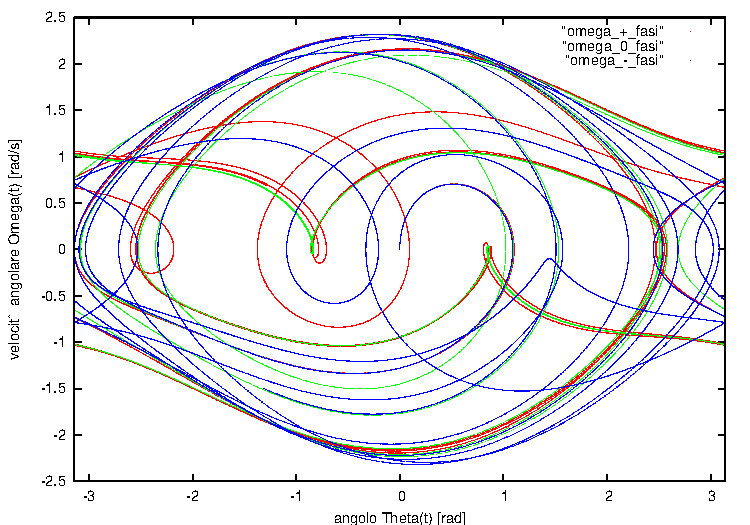
\includegraphics[width=13.5cm,keepaspectratio]{picture/chaos/confrontoomega_fasi}}
\end{figure}

\clearpage
\begin{thebibliography}{99}
\bibitem{recipe}\emph{Numerical recipes in C++}
\bibitem{knuth}Knuth D. \emph{The Art of Computer Programming}
\bibitem{hilde}Hildebrand F. \emph{Introduction to Numerical Analysis}, 2nd.ed.
\end{thebibliography}
\end{document}




